% certification/manual-content.tex
% Shared body: Chapter 0, Part I criterion chapters, Appendices A-E.
% Included by both edition shells.
% ============================================================================
% Chapter 0 --- Installation, Runtime Environment, and Configuration
% ============================================================================
\setcounter{chapter}{-1}
\chapter{Installation, Runtime Environment, and Configuration}
\label{chap:install}

\clearpage

This chapter records the exact environment, dependencies, and configuration
used to build the system and generate the certification test results in this
manual. Version numbers are drawn from the repository as of the commit cited in
the \hyperref[sec:reproducibility]{Reproducibility} section; treat that commit
plus \texttt{package-lock.json} as the authoritative build inputs.

\section{System Requirements}

\begin{table}[h]
\centering
\begin{tabular}{ll}
\toprule
\textbf{Component} & \textbf{Requirement} \\
\midrule
Operating system & macOS (Apple Silicon or Intel) for development; \\
                 & Linux (Debian/Ubuntu) for CI and production; \\
                 & Windows via WSL2 \\
Meteor           & 3.4 (\texttt{.meteor/release} = \texttt{METEOR@3.4}) \\
Node.js          & 22.22.0 --- bundled by Meteor 3.4 as the app runtime; \\
                 & a system Node $\geq$ 20 (CI uses 20.11.0) for npm / CLI tooling \\
MongoDB          & 6.0 or newer --- Meteor's bundled development Mongo is 7.0.16; \\
                 & CI runs the \texttt{mongo:6.0} image \\
Browser (E2E)    & Google Chrome / Chrome for Testing, with a version-matched \\
                 & ChromeDriver (the runs in this manual used 149.x) \\
Browser (app)    & Any modern evergreen browser (Chrome, Edge, Firefox, Safari) \\
Desktop (opt.)   & Electron via \texttt{npmPackages/desktop-lattice} --- not required \\
                 & for certification testing \\
\bottomrule
\end{tabular}
\caption{System requirements}
\end{table}

\section{Package Inventory}

Major dependencies, grouped by purpose. Versions are the declared ranges in
\texttt{package.json}; exact resolved versions are pinned in
\texttt{package-lock.json}.

\begin{longtable}{lll}
\toprule
\textbf{Purpose} & \textbf{Package} & \textbf{Version} \\
\midrule
\endfirsthead
\toprule
\textbf{Purpose} & \textbf{Package} & \textbf{Version} \\
\midrule
\endhead
\bottomrule
\endfoot
FHIR server      & (in-repo) \texttt{server/FhirEndpoints.js}, SearchParametersEngine & --- \\
                 & \texttt{@node-on-fhir/us-core} (US Core 7.0 profiles) & 7.0.0 \\
                 & \texttt{fhirpath} & 4.8.0 \\
\midrule
SMART / Auth     & \texttt{@node-oauth/express-oauth-server} & 4.1.5 \\
                 & \texttt{jsonwebtoken} & 9.0.2 \\
                 & \texttt{pkijs} + \texttt{asn1js} (X.509 / Backend Services) & 3.2.4 / 3.0.5 \\
                 & \texttt{bcrypt} & 6.0.0 \\
\midrule
Data / Mongo     & Meteor Mongo (server + Minimongo) & (Meteor 3.4) \\
                 & \texttt{simpl-schema}, \texttt{ajv} (FHIR JSON Schema) & --- / 8.20.0 \\
                 & \texttt{lodash}, \texttt{moment} & 4.18.1 / 2.29.4 \\
\midrule
Testing          & \texttt{nightwatch} (E2E) & 3.12.1 \\
                 & \texttt{chromedriver} & 146.0.6 \\
                 & \texttt{meteortesting:mocha} (unit) & (Meteor) \\
\midrule
UI               & \texttt{react} / \texttt{react-dom} & 18.2.0 \\
                 & \texttt{@mui/material} / \texttt{@mui/icons-material} & 5.16.7 \\
\midrule
C-CDA / QRDA     & \texttt{@node-on-fhir/ccda-export} (C-CDA gen + receive) & (in-repo) \\
                 & \texttt{@node-on-fhir/quality-measures} (QRDA I export) & (in-repo) \\
                 & \texttt{fqm-execution} (FHIR measure engine) & 1.8.5 \\
                 & \texttt{xml2js} (XML parse / build) & 0.6.2 \\
\midrule
Terminology      & CodeSystems / ValueSets collections + US Core profiles & --- \\
                 & code systems: CDCREC, LOINC, SNOMED CT, RxNorm (by reference) & --- \\
\midrule
DICOM            & \texttt{@cornerstonejs/core} & 1.78.0 \\
                 & \texttt{@cornerstonejs/dicom-image-loader} / \texttt{tools} & 1.78.0 \\
\midrule
Build tooling    & Meteor 3.4 bundler & 3.4 \\
                 & \texttt{@rspack/core} (Rspack) & 1.7.1 \\
                 & \texttt{tectonic} (LaTeX --- this manual only) & 0.16.x \\
\end{longtable}

\section{Installation}

Meteor is the prerequisite; it provisions the bundled Node and MongoDB.

\begin{lstlisting}
# 1. Install Meteor 3.x (once, system-wide)
curl https://install.meteor.com/ | sh

# 2. Clone and install
git clone https://github.com/node-on-fhir/core.git
cd core
npm install            # installs npm workspaces + symlinks workflow packages

# 3. Run (starts the app + bundled MongoDB on http://localhost:3000)
npm start              # equivalent to: meteor run
\end{lstlisting}

There is no separate \texttt{npm run dev} script; \texttt{npm start} maps to
\texttt{meteor run}. A first run compiles the bundle and may take several
minutes.

\section{Environment Variables}

The following variables configure the runtime; use safe placeholders in shared
environments and never commit real secrets. Development / test values:

\begin{lstlisting}
NODE_ENV=development                 # hard gate for dev auto-login
DEV_AUTO_LOGIN=true                  # enable dev auto-login
DEV_AUTO_USERNAME=demouser           # dev account username
DEV_AUTO_PASSWORD=<dev-password>     # dev account password (server-side only)
DEV_AUTO_PATIENT_ID=<fhir-id>        # optional: bind dev user to a Patient
TEST_RUN=1                           # gates destructive test-only operations
ENABLE_AUTOPUBLISH=true              # enable autopublish.* publications
INITIALIZE_SEARCH_PARAMETERS=true    # compile the FHIR SearchParametersEngine
                                     #   (REQUIRED for (g)(7)/(g)(9) search)
EXTRA_WORKFLOWS=@node-on-fhir/...    # comma-separated workflow packages to load
MONGO_URL=mongodb://localhost:27017/meteor   # override bundled dev Mongo
                                             #   (CI: mongodb://mongo:27017/meteor_test)
CHROMEDRIVER_PATH=/path/to/chromedriver      # match your local Chrome version
\end{lstlisting}

Server configuration that is not an environment variable is supplied via a
Meteor settings JSON file (\texttt{--settings}). Public keys land in
\texttt{Meteor.settings.public} (client-visible); private keys stay server-side.
Relevant fields (safe placeholders):

\begin{lstlisting}
{
  "public": {
    "title": "Care Commons",
    "fhirVersion": "R4",
    "devAutoLoginEnabled": true,
    "modules": {
      "patientDemographics": { "raceEthnicity": true }
    }
  },
  "private": {
    "fhir": {
      "rest": {
        "Patient": { "interactions": ["read","create","update","delete","search"],
                     "search": true, "publication": true }
      },
      "disableOauth": true
    },
    "accessControl": {
      "enableBasicAuth": false,
      "systemSecret": "<CHANGE-ME-do-not-commit>"
    }
  }
}
\end{lstlisting}

\textbf{Security note.} The certification/TDD settings file ships with
\texttt{disableOauth: true} so unauthenticated REST calls are granted a
\texttt{noauth} role --- convenient for a self-contained test run, but never a
production posture. Production deployments must enable OAuth / SMART, set a real
\texttt{systemSecret} (or migrate to JWT/JWK Backend Services), and keep
settings files containing secrets out of version control.

\section{Canonical Certification Configuration}
\label{sec:cert-config}

The certification test run in this manual was launched with the following exact
command --- environment variables, the workflow-package set, and the settings
file. This is the reproducible entry point for the whole suite:

\begin{lstlisting}
TEST_RUN=1 \
ENABLE_AUTOPUBLISH=true \
DEV_AUTO_LOGIN=true \
DEV_AUTO_USERNAME=demouser \
DEV_AUTO_PASSWORD=<dev-password> \
INITIALIZE_SEARCH_PARAMETERS=true \
EXTRA_WORKFLOWS=@node-on-fhir/order-catalog,@node-on-fhir/implantable-devices,@node-on-fhir/ccda-export,@node-on-fhir/prescription-benefit,@node-on-fhir/decision-support,@node-on-fhir/quality-measures,@node-on-fhir/secure-messaging \
  meteor run --settings settings/settings.honeycomb.tdd.json
\end{lstlisting}

The settings file \texttt{settings/settings.honeycomb.tdd.json} enables dev
auto-login, the per-resource FHIR REST interactions
(\texttt{private.fhir.rest.*}), and the race/ethnicity demographics gate
(\texttt{public.modules.patientDemographics.raceEthnicity = true}, required for
the (a)(5) test). Meteor reads \texttt{--settings} into \texttt{Meteor.settings}
at boot. The seven \texttt{EXTRA\_WORKFLOWS} packages supply the CPOE catalog,
implantable-device registry, C-CDA export/receive, real-time prescription
benefit, decision support, quality measures, and secure messaging surfaces
exercised by the criteria chapters.

\section{Test Execution}

Run the full Base EHR suite against a running server with the aggregate runner:

\begin{lstlisting}
./certification/tdd/base_ehr/run-base-ehr-tests.sh
\end{lstlisting}

Or run a single criterion directly (the form used to capture the per-chapter
results and screenshots in this manual):

\begin{lstlisting}
CHROMEDRIVER_PATH=/path/to/chromedriver \
  npx nightwatch --config nightwatch.circle.conf.js \
  certification/tdd/base_ehr/170.315.<x>.<y>.test.js
\end{lstlisting}

Each behavioral test drives real record / change / access behaviors against
FHIR resources per the ONC test procedures; a criterion is \textbf{Verified}
when its test passes green and a \textbf{Gap} when a test deliberately fails on a
documented missing capability. See the Certification Testing Notes appendix for
the full suite status and the relationship to Inferno.

\section{Reproducibility}
\label{sec:reproducibility}

The results, screenshots, and status table in this manual were generated with:

\begin{table}[h]
\centering
\begin{tabular}{ll}
\toprule
\textbf{Input} & \textbf{Value} \\
\midrule
Repository       & \texttt{github.com/node-on-fhir/core} (branch \texttt{baseehr-testcoverage}) \\
Commit SHA       & \texttt{c4ad354131cea9801a585b76ff04a629939eab24} \\
                 & (documentation-only changes may follow this commit) \\
\texttt{package-lock.json} & lockfileVersion 3; SHA-256 \\
                 & \texttt{a1a97949761c95fcde77784cc2a4c647ed9748443744c31965f7d3fd4a73782b} \\
                 & (4{,}121 locked packages, excluding the root project entry) \\
Node.js          & 22.22.0 (Meteor 3.4 runtime); 20.11.0 (CI tooling) \\
MongoDB          & 7.0.16 (bundled dev); 6.0 (CI) \\
Meteor           & 3.4 \\
Browser          & Chrome for Testing with version-matched ChromeDriver (149.x) \\
\bottomrule
\end{tabular}
\caption{Reproducibility inputs}
\end{table}

To reproduce, check out the commit above, restore dependencies from
\texttt{package-lock.json} with \texttt{npm ci}, launch with the
\hyperref[sec:cert-config]{Canonical Certification Configuration}, and run the
test-execution commands above.

% ============================================================================
\part{Base EHR Certification}
% ============================================================================

\chapter*{Overview}
\addcontentsline{toc}{chapter}{Overview}

This Part documents the Base EHR certification criteria per the ONC Health IT Certification Program, updated for the \textbf{CY2026 Base EHR definition} (45 CFR 170.102, as revised by the HTI final rules). The CPOE family (a)(1)--(a)(3) requires at least one member; the remaining rows are each required (some with future compliance dates, noted below).

\section*{Certification Criteria Summary}

The \textbf{Status} column reflects the outcome of the behavioral Nightwatch test suite under \texttt{certification/tdd/base\_ehr/} (one test file per criterion). \textbf{Verified} = the capability is built and its behavioral tests pass green. \textbf{Gap} = a behavioral test exists and deliberately fails on a documented missing capability (the suite is a live certification punch-list --- see the per-criterion chapters and the Certification Testing Notes appendix). \textbf{Inferno} = validated with the ONC-approved Inferno tool (previously run to green; to be re-run and formally recorded for ACB submission), not by this suite.

\textbf{Scope of the BDD feature files:} the embedded Gherkin features are the \emph{complete} behavioral specification for each criterion, and deliberately include forward-looking scenarios beyond the current regulatory floor (for example, the pronoun and inpatient mortality-data scenarios in (a)(5)). A criterion's \textbf{Verified} status attests to the scenarios exercised by its behavioral Nightwatch test, which may be a subset of the full feature file; the feature files are the specification, the tests are the evidence.

\begin{table}[h]
\centering
\begin{tabular}{lll}
\toprule
\textbf{Criterion} & \textbf{Title} & \textbf{Status} \\
\midrule
\textsection{} 170.315(a)(1) & CPOE - Medications & Verified \\
\textsection{} 170.315(a)(2) & CPOE - Laboratory & Verified \\
\textsection{} 170.315(a)(3) & CPOE - Diagnostic Imaging & Verified \\
\textsection{} 170.315(a)(5) & Demographics & Verified \\
\textsection{} 170.315(a)(14) & Implantable Device List & Verified \\
\textsection{} 170.315(b)(1) & Transitions of Care (C-CDA) & Verified \\
\textsection{} 170.315(b)(4) & Real-Time Prescription Benefit & Verified \\
\textsection{} 170.315(b)(11) & Decision Support Interventions & Verified \\
\textsection{} 170.315(c)(1) & Clinical Quality Measures - Record \& Export & Verified \\
\textsection{} 170.315(g)(7) & Application Access - Patient Selection & Verified \\
\textsection{} 170.315(g)(9) & Application Access - All Data Request & Verified \\
\textsection{} 170.315(g)(10) & Standardized API & Inferno \\
\textsection{} 170.315(h)(1) & Direct Project (or (h)(2)) & Gap \\
\bottomrule
\end{tabular}
\caption{CY2026 Base EHR Certification Criteria --- test-verified status (11 verified, 1 documented gap, 1 external/Inferno)}
\end{table}

\textbf{The remaining documented gap} is (h)(1) Direct messaging, which has no operational transport (SMTP/S-MIME/HISP) and uses simulated certificate trust; it is detailed in its chapter and tracked in the project's engineering ledger. The former (a)(5), (b)(1), and (c)(1) gaps have since been remediated: (a)(5) now records race/ethnicity per CDCREC as US~Core extensions (settings-gated --- see that chapter); (b)(1) now populates the C-CDA from the real patient record and adds an inbound receive/validate/display path; and (c)(1) now exports a QRDA Category~I document per \textsection{} 170.205(h)(2).

\textbf{Note on future compliance dates:} (b)(4) Real-Time Prescription Benefit is an HTI-4 criterion required by 1/1/2028, and (b)(11) Decision Support Interventions has a Privacy \& Security update due 12/31/2027. Both are tested at their current baseline; absent future-dated portions are treated as informational, not gaps.

\textbf{Legacy / non-core criteria documented separately:} \textsection{} 170.315(a)(4) Drug Interaction Checks, \textsection{} 170.315(a)(9) Clinical Decision Support (\textbf{expired} 1/1/2025, replaced by (b)(11)), and \textsection{} 170.315(e)(1) View, Download, Transmit are retained as reference chapters below but are not part of the CY2026 Base EHR core set above.

% ============================================================================
\chapter{\textsection{} 170.315(a)(1) - CPOE Medications}
\label{chap:a1}
% ============================================================================

\clearpage

\section{Criterion Information}

\subsection{Maturity Level}
\maturitylabel{verified}

\subsection{Regulatory Text}

From \textit{45 CFR \textsection{} 170.315(a)(1)}:

\begin{quotation}
\textbf{(1) Computerized provider order entry---medications.}

\textbf{(i)} Enable a user to record, change, and access medication orders.

\textbf{(ii)} Optional. Include a ``reason for order'' field.
\end{quotation}

\section{Behavior-Driven Development Specification}

\lstinputlisting[language=Gherkin, caption={170.315(a)(1) - CPOE Medications}]{bdd/170.315-a-1-cpoe-medications.feature}

\section{Screenshots}

\begin{figure}[h]
\centering
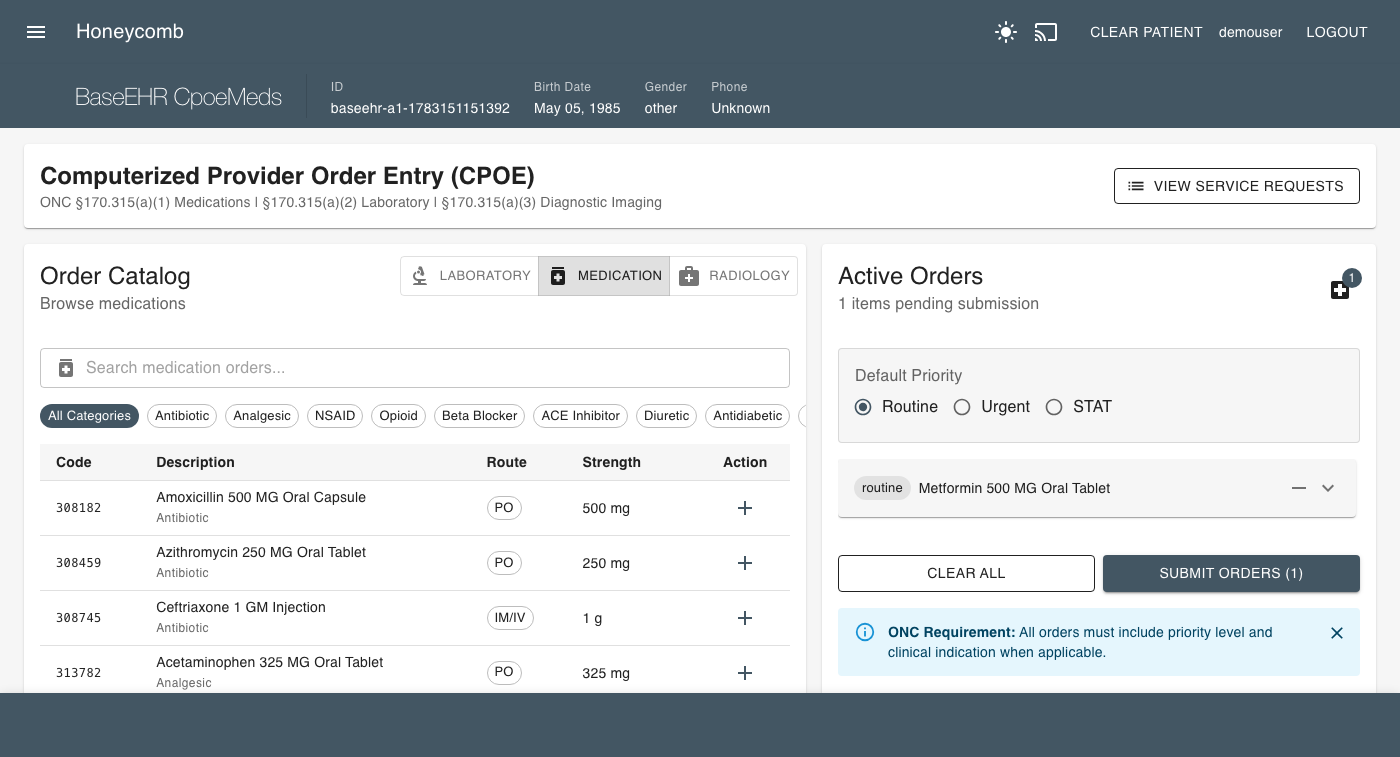
\includegraphics[width=\textwidth]{screenshots/base-ehr_170.315.a.1_cpoe-medications.png}
\caption{CPOE Medications - Order Entry Interface}
\label{fig:a1-screenshot}
\end{figure}

% ============================================================================
\chapter{\textsection{} 170.315(a)(2) - CPOE Laboratory}
\label{chap:a2}
% ============================================================================

\clearpage

\section{Criterion Information}

\subsection{Maturity Level}
\maturitylabel{verified}

\subsection{Regulatory Text}

From \textit{45 CFR \textsection{} 170.315(a)(2)}:

\begin{quotation}
\textbf{(2) Computerized provider order entry---laboratory.}

\textbf{(i)} Enable a user to record, change, and access laboratory orders.

\textbf{(ii)} Optional. Include a ``reason for order'' field.
\end{quotation}

\section{Behavior-Driven Development Specification}

\lstinputlisting[language=Gherkin, caption={170.315(a)(2) - CPOE Laboratory}]{bdd/170.315-a-2-cpoe-laboratory.feature}

\section{Screenshots}

\begin{figure}[h]
\centering
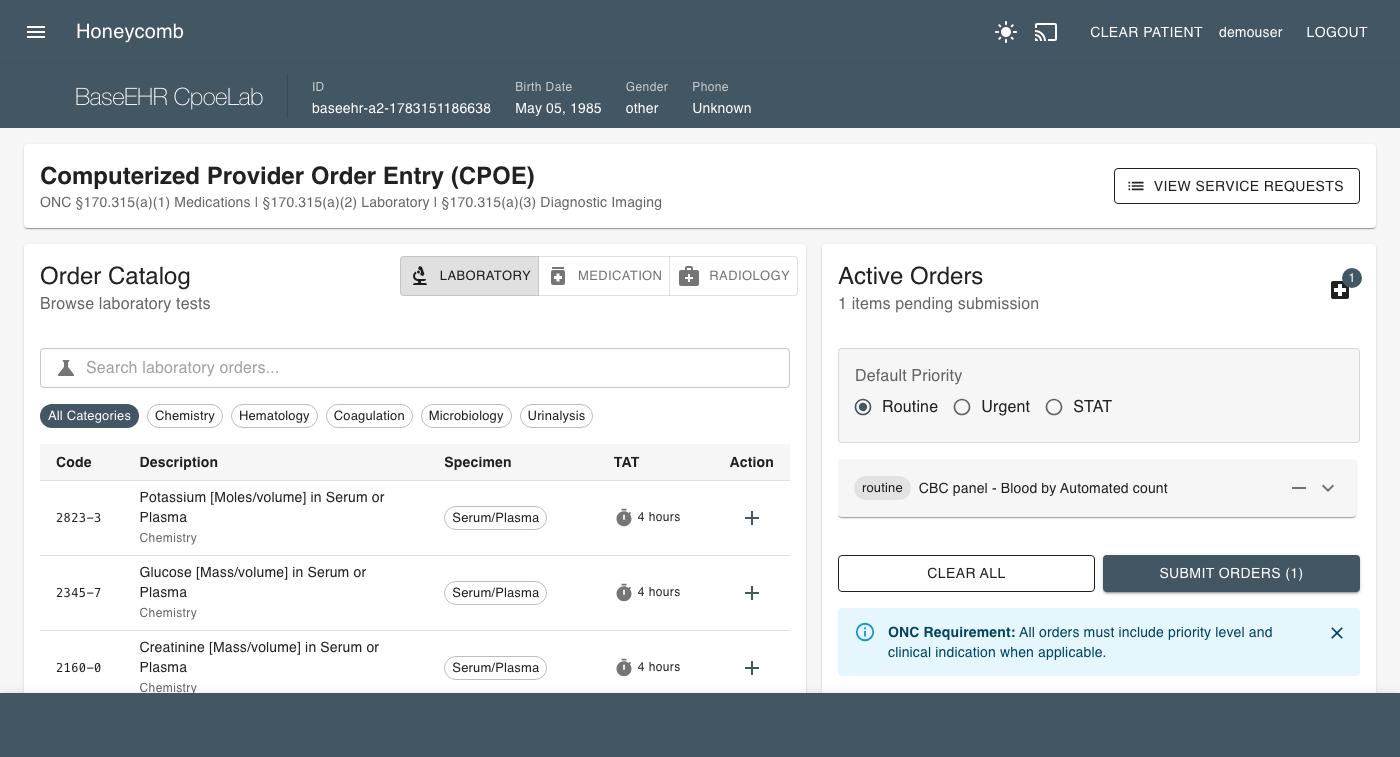
\includegraphics[width=\textwidth]{screenshots/base-ehr_170.315.a.2_cpoe-laboratory.png}
\caption{CPOE Laboratory - Order Entry Interface}
\label{fig:a2-screenshot}
\end{figure}

% ============================================================================
\chapter{\textsection{} 170.315(a)(3) - CPOE Diagnostic Imaging}
\label{chap:a3}
% ============================================================================

\clearpage

\section{Criterion Information}

\subsection{Maturity Level}
\maturitylabel{verified}

\subsection{Regulatory Text}

From \textit{45 CFR \textsection{} 170.315(a)(3)}:

\begin{quotation}
\textbf{(3) Computerized provider order entry---diagnostic imaging.}

\textbf{(i)} Enable a user to record, change, and access diagnostic imaging orders.

\textbf{(ii)} Optional. Include a ``reason for order'' field.
\end{quotation}

\section{Behavior-Driven Development Specification}

\lstinputlisting[language=Gherkin, caption={170.315(a)(3) - CPOE Diagnostic Imaging}]{bdd/170.315-a-3-cpoe-diagnostic-imaging.feature}

\section{Screenshots}

\begin{figure}[h]
\centering
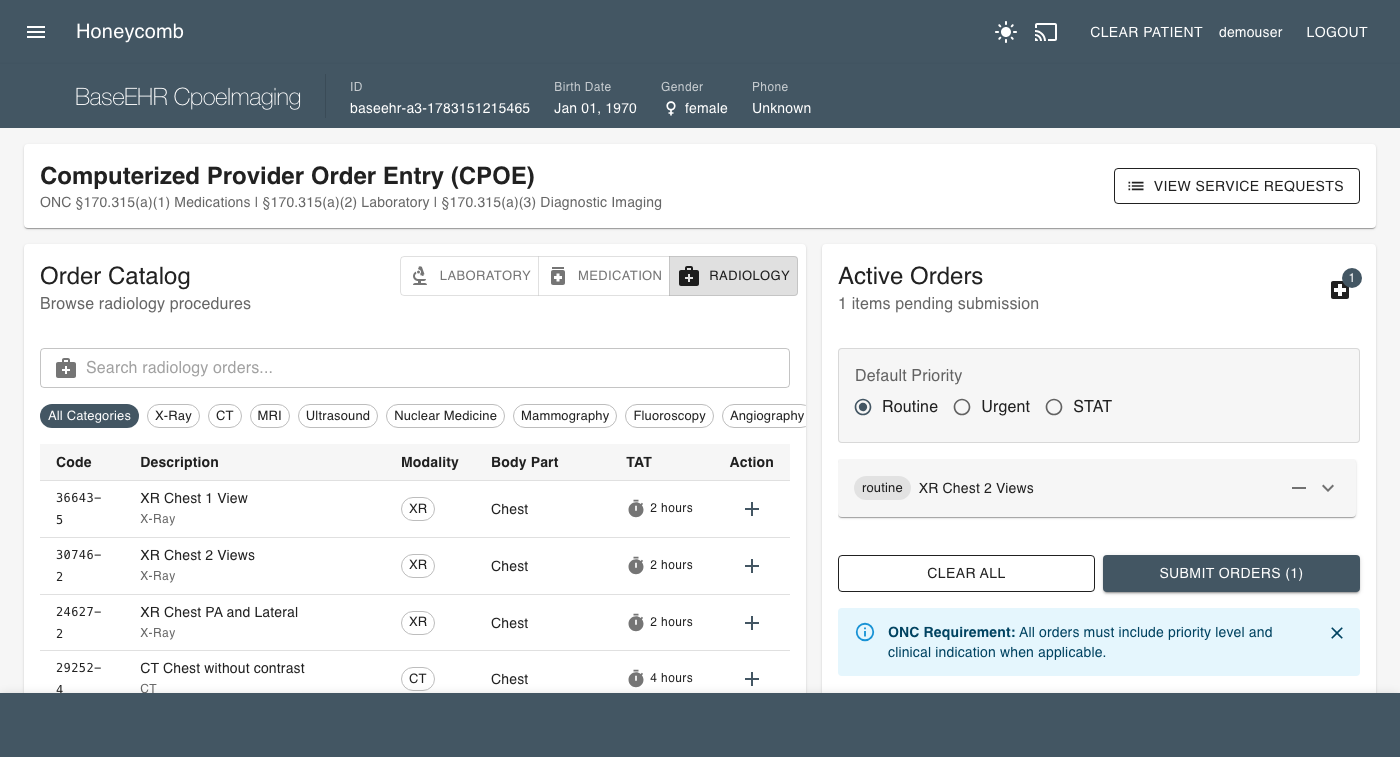
\includegraphics[width=\textwidth]{screenshots/base-ehr_170.315.a.3_cpoe-diagnostic-imaging.png}
\caption{CPOE Diagnostic Imaging - Order Entry Interface}
\label{fig:a3-screenshot}
\end{figure}

% ============================================================================
\chapter{\textsection{} 170.315(a)(4) - Drug Interaction Checks}
\label{chap:a4}
% ============================================================================

\clearpage

\section{Criterion Information}

\subsection{Maturity Level}
\maturitylabel{implemented}

\subsection{Regulatory Text}

From \textit{45 CFR \textsection{} 170.315(a)(4)}:

\begin{quotation}
\textbf{(4) Drug-drug, drug-allergy interaction checks for CPOE ---}

\textbf{(i) Interventions.} Before a medication order is completed and acted upon during computerized provider order entry (CPOE), interventions must automatically indicate to a user drug-drug and drug-allergy contraindications based on a patient's medication list and medication allergy list.

\textbf{(ii) Adjustments.}

\textbf{(A)} Enable the severity level of interventions provided for drug-drug interaction checks to be adjusted.

\textbf{(B)} Limit the ability to adjust severity levels in at least one of these two ways:

\textbf{(1)} To a specific set of identified users.

\textbf{(2)} As a system administrative function.
\end{quotation}

\section{Behavior-Driven Development Specification}

\lstinputlisting[language=Gherkin, caption={170.315(a)(4) - Drug Interaction Checks}]{bdd/170.315-a-4-drug-interactions.feature}

% No screenshot: (a)(4) is retained as a non-core reference chapter (not part
% of the CY2026 Base EHR core set); a real test-run capture will be added if
% the criterion enters certification scope.

% ============================================================================
\chapter{\textsection{} 170.315(a)(5) - Demographics}
\label{chap:a5}
% ============================================================================

\clearpage

\section{Criterion Information}

\subsection{Maturity Level}
\maturitylabel{verified}

\subsection{Regulatory Text}

From \textit{45 CFR \textsection{} 170.315(a)(5)}:

\begin{quotation}
\textbf{(5) Patient demographics and observations.}

\textbf{(i)} Enable a user to record, change, and access patient demographic and observations data including race, ethnicity, preferred language, sex, sex parameter for clinical use, sexual orientation, gender identity, name to use, pronouns, and date of birth.
\end{quotation}

(Full regulatory text abbreviated for brevity. See BDD specification for complete requirements.)

\subsection{Implementation}

The behavioral test records, changes, and accesses name, date of birth, sex (US~Core birth-sex, with a decline-to-specify option), and preferred language (RFC~5646), and now \textbf{race and ethnicity} per the CDCREC code system aggregated to OMB categories, with a declined-to-specify option. The patient form provides multi-select Race and Ethnicity fields, and the patient-write methods preserve the complex (nested sub-extension) US~Core \texttt{us-core-race} / \texttt{us-core-ethnicity} extensions.

\textbf{Settings gate (international deployments):} collecting race/ethnicity is legally forbidden in some jurisdictions, so it is opt-in --- the fields render, and the extensions persist, only when \texttt{settings.public.modules.patientDemographics.raceEthnicity} is enabled; when disabled the fields are hidden and the server strips the extensions defensively. US certification builds enable the flag.

\textbf{Regulatory note (CCG v1.3, updated 05/2026):} consistent with Executive Order 14168 and OPM guidance, sexual orientation, gender identity, sex parameter for clinical use, name to use, and pronouns are \emph{not} required for (a)(5); the sex requirement reduces to recording Female or Male (plus decline).

\section{Behavior-Driven Development Specification}

\lstinputlisting[language=Gherkin, caption={170.315(a)(5) - Demographics}]{bdd/170.315-a-5-demographics-observations.feature}

\section{Screenshots}

\begin{figure}[h]
\centering
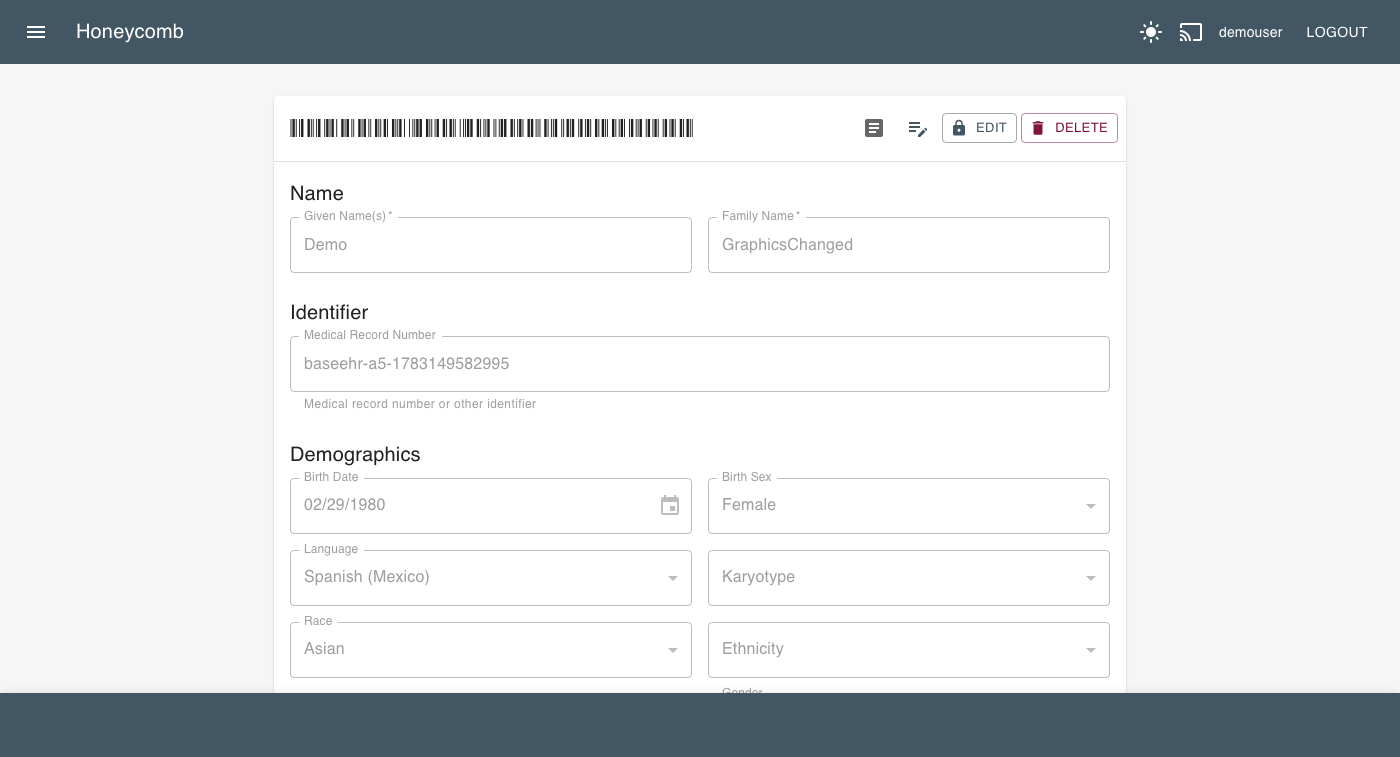
\includegraphics[width=\textwidth]{screenshots/base-ehr_170.315.a.5_demographics.png}
\caption{Patient Demographics - Data Entry Interface}
\label{fig:a5-screenshot}
\end{figure}

% ============================================================================
\chapter{\textsection{} 170.315(a)(9) - Clinical Decision Support (EXPIRED)}
\label{chap:a9}
% ============================================================================

\clearpage

\section{Criterion Information}

\subsection{Maturity Level}
\maturitylabel{implemented} \textbf{(EXPIRED)}

\subsection{Expiration Notice}

\textcolor{red}{\textbf{CRITICAL: This criterion EXPIRED on January 1, 2025 per 45 CFR \textsection{} 170.315(a)(9)(vi).}}

This criterion has been replaced by \textsection{} 170.315(b)(11) - Decision Support Interventions (see Chapter \ref{chap:b11}).

Due to government website unavailability as of January 2025, it is unclear whether Base EHR certifications issued before the expiration date can still use this criterion (grandfathered), or if all certifications must now use \textsection{} 170.315(b)(11).

\subsection{Regulatory Text}

From \textit{45 CFR \textsection{} 170.315(a)(9)}:

\begin{quotation}
\textbf{(9) Clinical decision support (CDS) ---}

\textbf{(i) CDS intervention interaction.} Interventions provided to a user must occur when a user is interacting with technology.

(Full regulatory text abbreviated. See BDD specification for complete requirements.)

\textbf{(vi) Expiration of criterion.} The adoption of this criterion for purposes of the ONC Health IT Certification Program expires on January 1, 2025.
\end{quotation}

\section{Behavior-Driven Development Specification}

\lstinputlisting[language=Gherkin, caption={170.315(a)(9) - Clinical Decision Support}]{bdd/170.315-a-9-clinical-decision-support.feature}

% No screenshot: (a)(9) EXPIRED 1/1/2025 and is retained only as a historical
% reference chapter; its successor (b)(11) carries the real test-run capture.

% ============================================================================
\chapter{\textsection{} 170.315(b)(1) - Transitions of Care}
\label{chap:b1}
% ============================================================================

\clearpage

\section{Criterion Information}

\subsection{Maturity Level}
\maturitylabel{verified}

\subsection{Regulatory Text}

From \textit{45 CFR \textsection{} 170.315(b)(1)}:

\begin{quotation}
\textbf{(1) Transitions of care.}

\textbf{(i) Send and receive via Edge Protocol.} Send and receive transition-of-care/referral summaries formatted per the Consolidated CDA (C-CDA) Release~2.1, using an Edge Protocol.

\textbf{(ii) Validate and display.} Validate received C-CDA documents against the standard and display their contents.

\textbf{(iii) Create.} Create a transition-of-care/referral summary as a C-CDA document, populated from the patient's record per the Common Clinical Data Set / USCDI.
\end{quotation}

(Full regulatory text abbreviated. See BDD specification for complete requirements.)

\subsection{Implementation}

The behavioral test verifies create, validate, access, and receive: a C-CDA~R2.1-enveloped transition-of-care document (Transfer Summary, LOINC~18761-7) is generated with the US~Realm header, CCD template identifiers, and LOINC-coded Allergies/Medications/Problems sections, \textbf{populated from the real patient record} (the document gathers Patients, AllergyIntolerances, MedicationRequests/Statements, Conditions, Observations, and Procedures for the patient); it is persisted as a FHIR \texttt{DocumentReference} with the XML as a base64 attachment plus an \texttt{AuditEvent}; and a malformed document is rejected by the validator.

An \textbf{inbound receive} path (\texttt{clinicalDocuments.receiveCCDA}) parses an externally-authored C-CDA (via XML parsing), validates the envelope, extracts patient demographics and the section list, and stores it for display in the Clinical Documents list/detail; a Receive~C-CDA upload control is provided on the export page. Structured-entry \emph{incorporation} (creating Conditions/etc.\ from parsed sections) and schematron-grade validation are flagged follow-ons.

\section{Behavior-Driven Development Specification}

\lstinputlisting[language=Gherkin, caption={170.315(b)(1) - Transitions of Care}]{bdd/170.315-b-1-transitions-of-care.feature}

\section{Screenshots}

\begin{figure}[h]
\centering
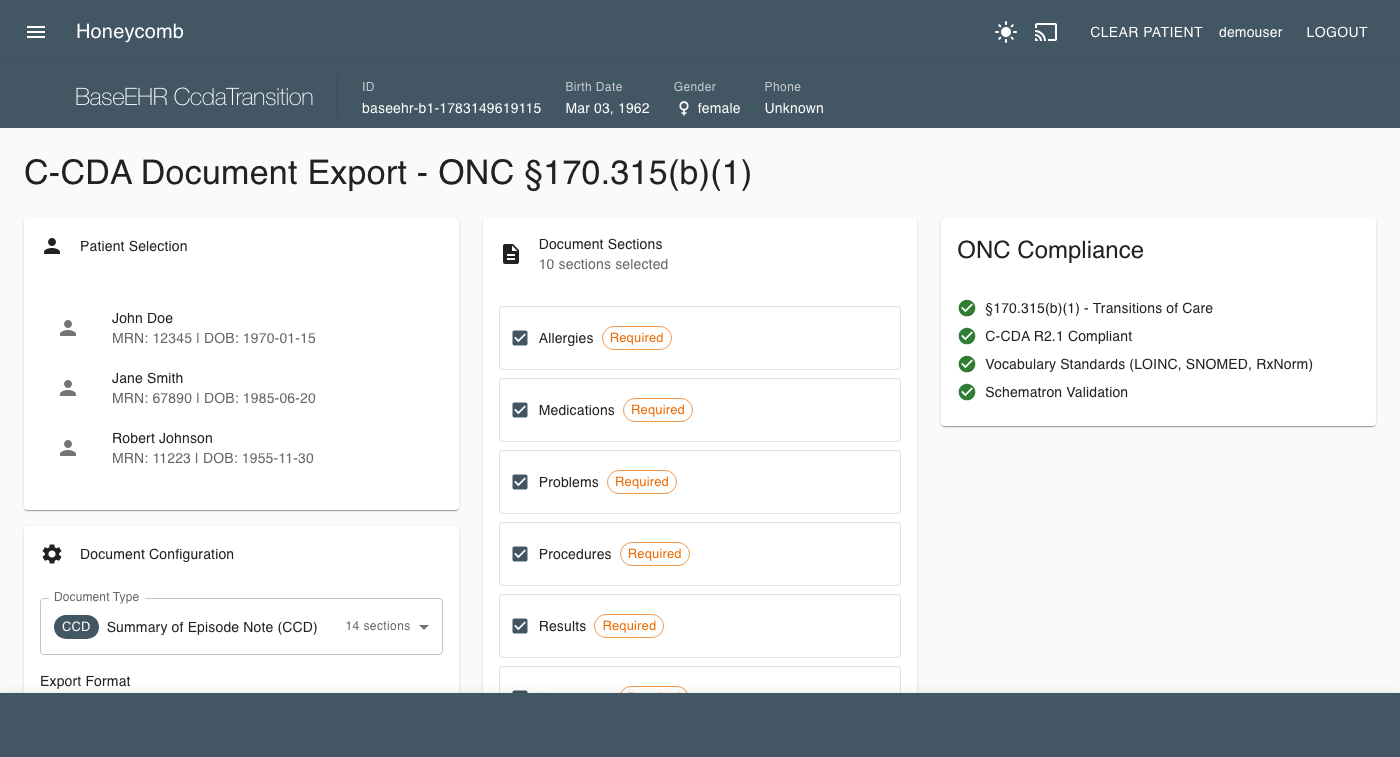
\includegraphics[width=\textwidth]{screenshots/base-ehr_170.315.b.1_transitions-of-care.png}
\caption{Transitions of Care - C-CDA Generation}
\label{fig:b1-screenshot}
\end{figure}

% ============================================================================
\chapter{\textsection{} 170.315(b)(4) - Real-Time Prescription Benefit}
\label{chap:b4}
% ============================================================================

\clearpage

\section{Criterion Information}

\subsection{Maturity Level}
\maturitylabel{verified}

\subsection{Regulatory Text}

From \textit{45 CFR \textsection{} 170.315(b)(4)}:

\begin{quotation}
\textbf{(4) Real-time prescription benefit (RTPB).}

Enable a user, for a prescribed drug, to request and receive real-time prescription benefit information --- including patient cost, formulary/coverage status, and any therapeutic alternatives --- from a benefit source.
\end{quotation}

(Full regulatory text abbreviated. See BDD specification for complete requirements.)

\subsection{Implementation Status}

The behavioral test drives the full RTPB round-trip: it composes an \texttt{RTPBRequest} for a prescribed product, transacts it against a benefit responder (a formulary/PBM responder from the responder registry), and receives an \texttt{RTPBResponse} carrying the patient's cost and cheaper therapeutic alternatives (a brand statin returns generic substitutions). Both request and response XML are rendered and persisted with request/response linkage, and the completed check appears in the transaction history. A configurable live endpoint is supported alongside the built-in certification-evidence responders.

\textbf{Future compliance date:} (b)(4) is an HTI-4 criterion required by 1/1/2028. The current baseline (request/response, patient cost, alternatives, live-endpoint capability) is verified; the final standard-version binding is treated as informational until closer to the compliance date, not a gap.

\section{Behavior-Driven Development Specification}

A dedicated Gherkin feature file for (b)(4) is not yet authored; the executable specification is the behavioral Nightwatch test \texttt{certification/tdd/base\_ehr/170.315.b.4.test.js}, which drives the request/response round-trip, patient-cost and therapeutic-alternative assertions, and the transaction-history retrieval described above.

\section{Screenshots}

\begin{figure}[h]
\centering
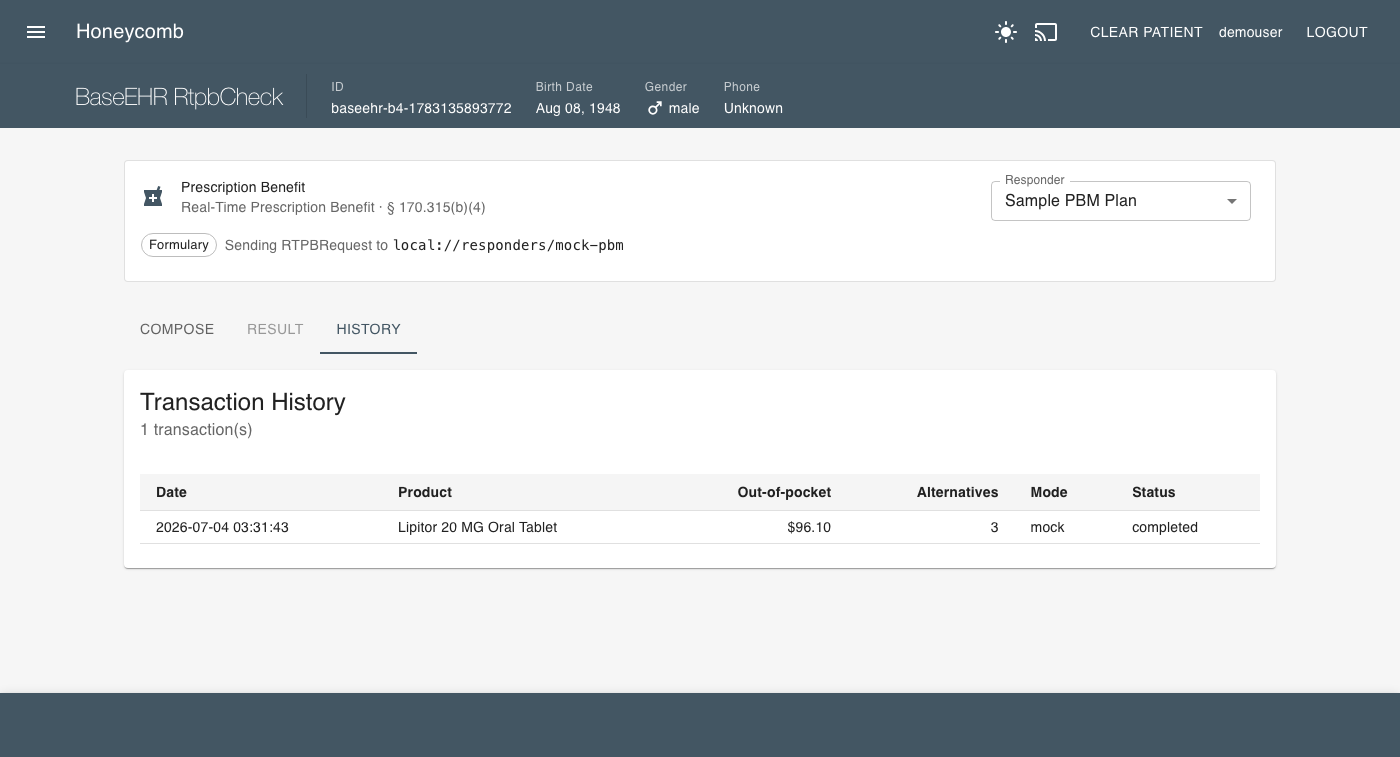
\includegraphics[width=\textwidth]{screenshots/base-ehr_170.315.b.4_prescription-benefit.png}
\caption{Real-Time Prescription Benefit - Cost and Alternatives}
\label{fig:b4-screenshot}
\end{figure}

% ============================================================================
\chapter{\textsection{} 170.315(b)(11) - Decision Support Interventions}
\label{chap:b11}
% ============================================================================

\clearpage

\section{Criterion Information}

\subsection{Maturity Level}
\maturitylabel{verified}

\subsection{Replacement Notice}

\textbf{This criterion REPLACES \textsection{} 170.315(a)(9) which expired January 1, 2025.}

Decision Support Interventions (DSI) is an enhanced version of the legacy Clinical Decision Support criterion, adding requirements for:
\begin{itemize}
\item Predictive decision support interventions (AI/ML algorithms)
\item Demographic data usage transparency
\item Electronic intervention feedback mechanism
\item Enhanced risk and fairness disclosures for predictive DSI
\end{itemize}

\subsection{Regulatory Text}

From \textit{45 CFR \textsection{} 170.315(b)(11)}:

\begin{quotation}
\textbf{(11) Decision Support Interventions.}

(Full regulatory text includes all requirements from a-9 plus enhanced requirements for predictive interventions, demographic transparency, feedback mechanisms, and algorithm governance. See BDD specification for complete requirements.)
\end{quotation}

\section{Behavior-Driven Development Specification}

\lstinputlisting[language=Gherkin, caption={170.315(b)(11) - Decision Support Interventions}]{bdd/170.315-b-11-decision-support-interventions.feature}

\section{Screenshots}

\begin{figure}[h]
\centering
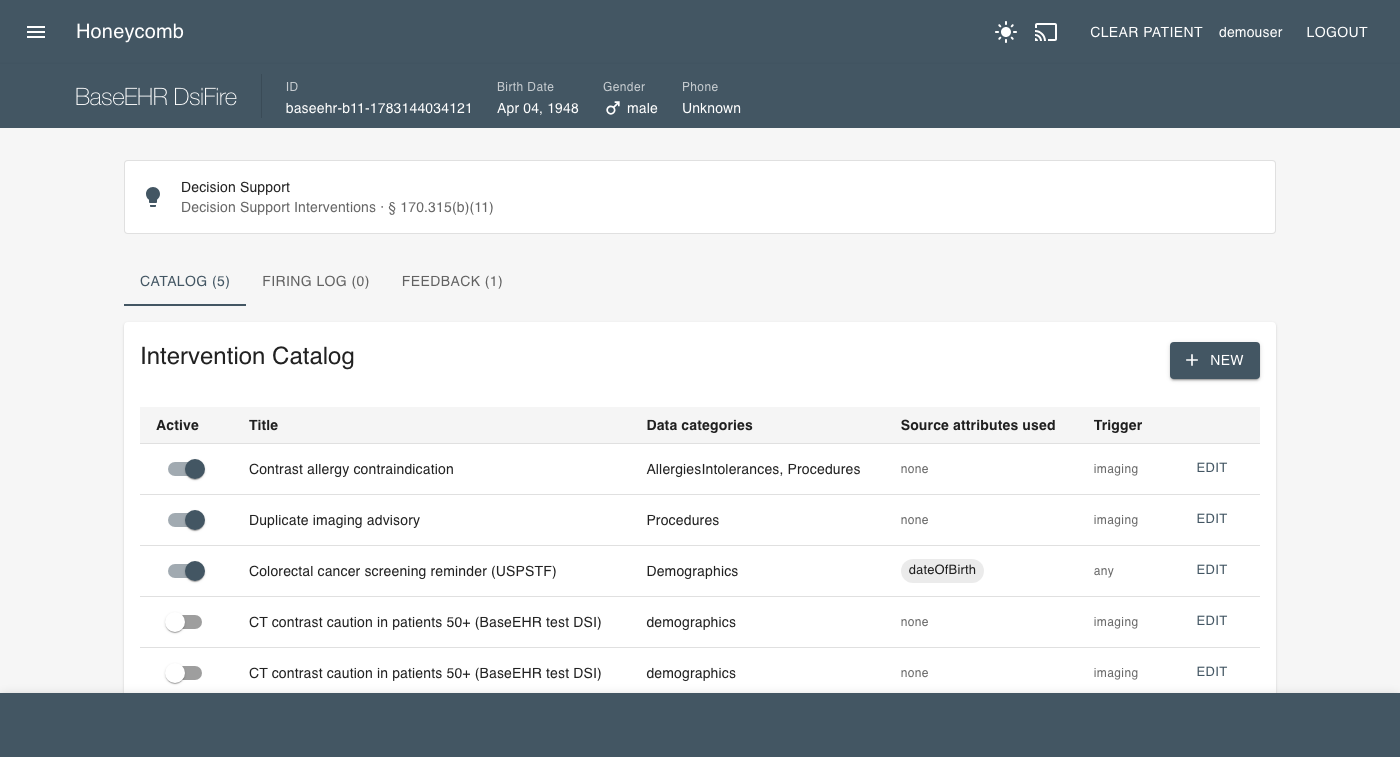
\includegraphics[width=\textwidth]{screenshots/base-ehr_170.315.b.11_decision-support.png}
\caption{Decision Support Interventions - Configuration Interface}
\label{fig:b11-screenshot}
\end{figure}

% ============================================================================
\chapter{\textsection{} 170.315(a)(14) - Implantable Device List}
\label{chap:a14}
% ============================================================================

\clearpage

\section{Criterion Information}

\subsection{Maturity Level}
\maturitylabel{verified}

\subsection{Regulatory Text}

From \textit{45 CFR \textsection{} 170.315(a)(14)}:

\begin{quotation}
\textbf{(14) Implantable device list.}

\textbf{(i)} Record Unique Device Identifiers associated with a patient's Implantable Devices.

\textbf{(ii)} Parse the following identifiers from a Unique Device Identifier.

(Full regulatory text abbreviated. See BDD specification for complete requirements.)
\end{quotation}

\section{Behavior-Driven Development Specification}

\lstinputlisting[language=Gherkin, caption={170.315(a)(14) - Implantable Device List}]{bdd/170.315-a-14-implantable-device-list.feature}

\section{Screenshots}

\begin{figure}[h]
\centering
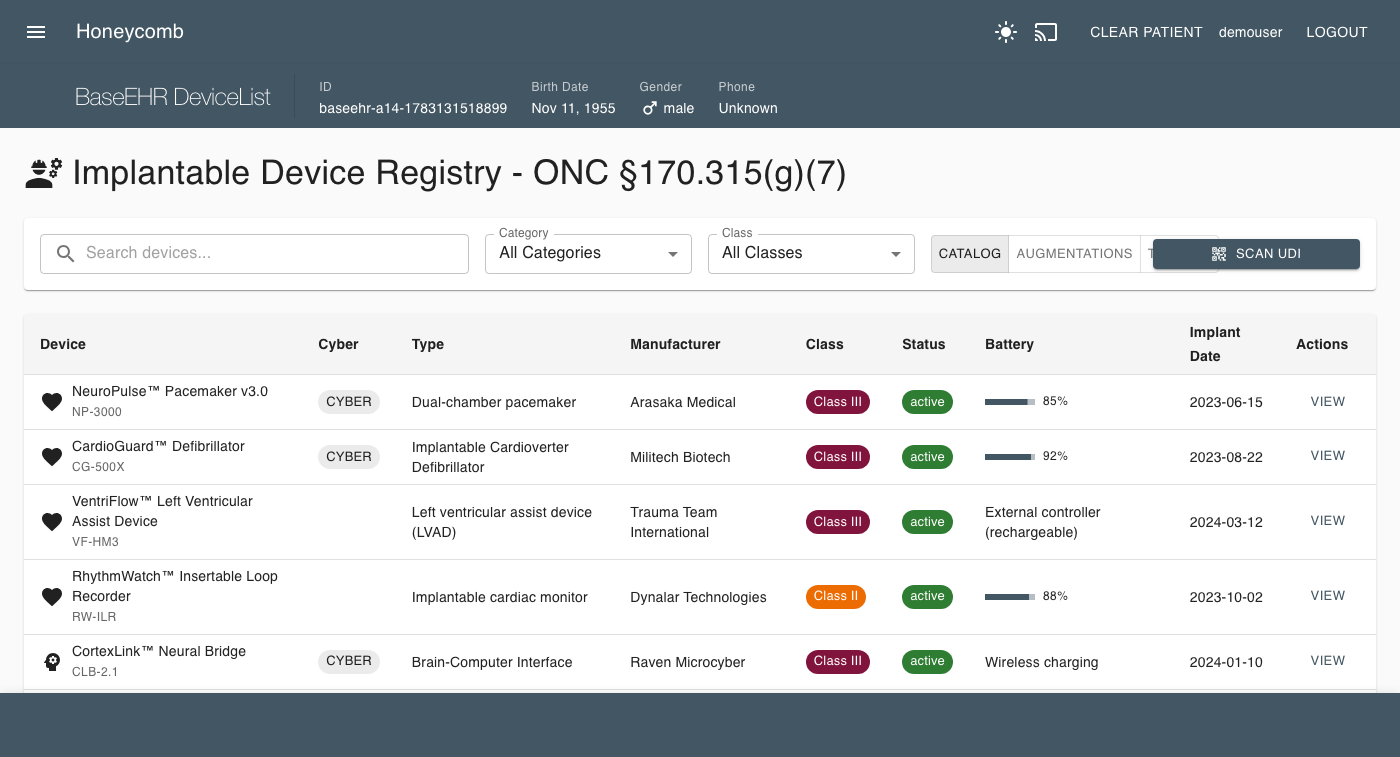
\includegraphics[width=\textwidth]{screenshots/base-ehr_170.315.a.14_implantable-devices.png}
\caption{Implantable Device List - Patient View}
\label{fig:a14-screenshot}
\end{figure}

% ============================================================================
\chapter{\textsection{} 170.315(e)(1) - View, Download, Transmit}
\label{chap:e1}
% ============================================================================

\clearpage

\section{Criterion Information}

\subsection{Maturity Level}
\maturitylabel{implemented}

\subsection{Regulatory Text}

From \textit{45 CFR \textsection{} 170.315(e)(1)}:

\begin{quotation}
\textbf{(1) View, download, and transmit to 3rd party.}

The technology must enable patients to view, download, and transmit their health information.

(Full regulatory text abbreviated. See BDD specification for complete requirements.)
\end{quotation}

\section{Behavior-Driven Development Specification}

\lstinputlisting[language=Gherkin, caption={170.315(e)(1) - View, Download, Transmit}]{bdd/170.315-e-1-view-download-transmit.feature}

% No screenshot: (e)(1) is retained as a non-core reference chapter (not part
% of the CY2026 Base EHR core set); a real test-run capture will be added if
% the criterion enters certification scope.

% ============================================================================
\chapter{\textsection{} 170.315(g)(7) - Application Access - Patient Selection}
\label{chap:g7}
% ============================================================================

\clearpage

\section{Criterion Information}

\subsection{Maturity Level}
\maturitylabel{verified}

\subsection{Regulatory Text}

From \textit{45 CFR \textsection{} 170.315(g)(7)}:

\begin{quotation}
\textbf{(7) Application access---patient selection.}

The technology must be able to receive a request with sufficient information to uniquely identify a patient and return an ID or other token.

(Full regulatory text abbreviated. See BDD specification for complete requirements.)
\end{quotation}

\section{Behavior-Driven Development Specification}

\lstinputlisting[language=Gherkin, caption={170.315(g)(7) - Application Access}]{bdd/170.315-g-7-10-apis.feature}

% No screenshot: (g)(7) is a FHIR REST API criterion with no user interface;
% conformance is exercised by the behavioral API test and validated via Inferno.

% ============================================================================
\chapter{\textsection{} 170.315(g)(9) - Application Access - All Data}
\label{chap:g9}
% ============================================================================

\clearpage

\section{Criterion Information}

\subsection{Maturity Level}
\maturitylabel{verified}

\subsection{Regulatory Text}

From \textit{45 CFR \textsection{} 170.315(g)(9)}:

\begin{quotation}
\textbf{(9) Application access---all data request.}

Provide an application programming interface (API) that can return all available data for a specific patient in a single request.

(Full regulatory text abbreviated. See BDD specification for complete requirements.)
\end{quotation}

\section{Behavior-Driven Development Specification}

\lstinputlisting[language=Gherkin, caption={170.315(g)(9) - Application Access}]{bdd/170.315-g-7-10-apis.feature}

% No screenshot: (g)(9) is a FHIR REST API criterion ($everything) with no user
% interface; conformance is exercised by the behavioral API test and validated
% via Inferno.

% ============================================================================
\chapter{\textsection{} 170.315(g)(10) - Standardized API}
\label{chap:g10}
% ============================================================================

\clearpage

\section{Criterion Information}

\subsection{Maturity Level}
\maturitylabel{implemented}

\subsection{Regulatory Text}

From \textit{45 CFR \textsection{} 170.315(g)(10)}:

\begin{quotation}
\textbf{(10) Standardized API for patient and population services.}

The technology must implement a standardized API that conforms to FHIR R4, US Core, SMART App Launch, OpenID Connect, and SMART Backend Services.

(Full regulatory text abbreviated. See BDD specification for complete requirements.)
\end{quotation}

\subsection{Inferno Validation Status}

Conformance for this criterion is established by the ONC-approved
\textbf{Inferno} testing tool, not by the in-repo behavioral suite. The
Inferno (g)(10) Standardized API test suite has been run against this system
with passing results; a refreshed run will be executed and its results
formally recorded as part of an ACB submission. Until certification is
issued by an ONC-ACB, this status represents validation evidence, not a
certification claim.

\section{Behavior-Driven Development Specification}

\lstinputlisting[language=Gherkin, caption={170.315(g)(10) - Standardized API}]{bdd/170.315-g-7-10-apis.feature}

% No screenshot: (g)(10) is the Standardized API criterion (FHIR R4 / US Core /
% SMART App Launch / OpenID Connect / SMART Backend Services) with no bespoke UI;
% conformance is validated externally with the ONC-approved Inferno tool.

% ============================================================================
\chapter{\textsection{} 170.315(c)(1) - Clinical Quality Measures - Record and Export}
\label{chap:c1}
% ============================================================================

\clearpage

\section{Criterion Information}

\subsection{Maturity Level}
\maturitylabel{verified}

\subsection{Regulatory Text}

From \textit{45 CFR \textsection{} 170.315(c)(1)}:

\begin{quotation}
\textbf{(1) Clinical quality measures --- record and export.}

\textbf{(i) Record.} For each clinical quality measure (CQM) presented for certification, record all of the data identified in the standard necessary to calculate the measure.

\textbf{(ii) Export.} Enable a user to electronically export a data file, for one or more patients, formatted per the QRDA Category~I standard (45 CFR 170.205(h)(2)), that includes all of the recorded CQM data.
\end{quotation}

(Full regulatory text abbreviated. See BDD specification for complete requirements.)

\subsection{Implementation}

The behavioral test verifies the record-calculate-export pipeline: the measures catalog is populated (seeded CMS/PACIO measures); a numerator event is recorded as a measure-observation-profiled FHIR \texttt{Observation}; an individual FHIR \texttt{MeasureReport} is calculated (fqm-execution / PACIO evaluators) with initial-population, denominator, and numerator groups and persisted; and the captured reports export as a FHIR Bundle, CSV, JSON, \textbf{and QRDA Category~I} (\textsection{} 170.205(h)(2)). The QRDA~I export produces a patient-level CDA document with the QRDA Category~I template identifiers and Measure, Reporting Parameters, and Patient Data sections, built from the patient's real demographics and the measure's population results.

\textbf{Scope:} the QRDA~I document is real and standards-shaped (correct envelope, template identifiers, and sections). Full per-measure QDM data-criteria entry coverage validated by the Cypress tool is the remaining external certification work; QRDA Category~III (for (c)(3)) is a follow-on.

\section{Behavior-Driven Development Specification}

\lstinputlisting[language=Gherkin, caption={170.315(c)(1) - CQM Record and Export}]{bdd/170.315-c-1-cqm-record-export.feature}

\section{Screenshots}

\begin{figure}[h]
\centering
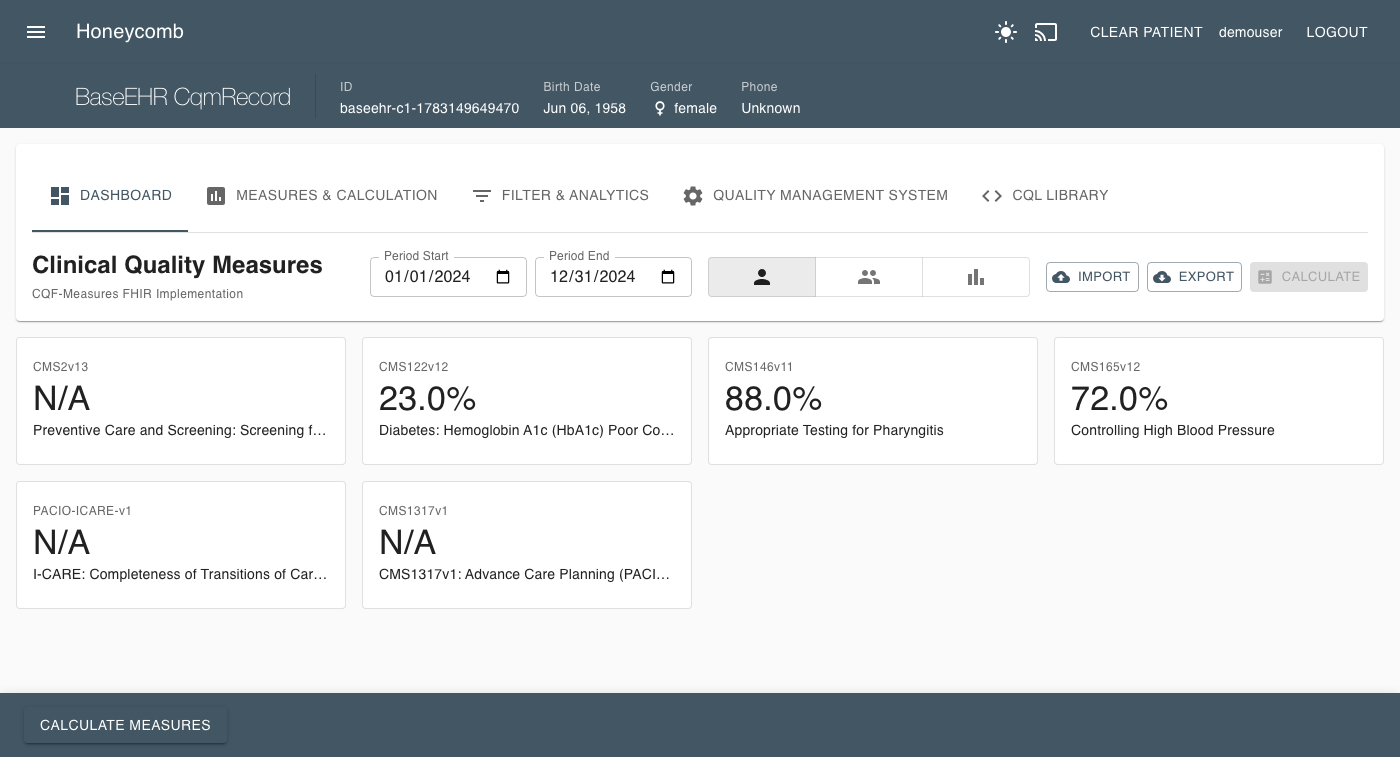
\includegraphics[width=\textwidth]{screenshots/base-ehr_170.315.c.1_quality-measures.png}
\caption{Clinical Quality Measures - Record and Export}
\label{fig:c1-screenshot}
\end{figure}

% ============================================================================
\chapter{\textsection{} 170.315(h)(1) - Direct Project}
\label{chap:h1}
% ============================================================================

\clearpage

\section{Criterion Information}

\subsection{Maturity Level}
\maturitylabel{gap}

\subsection{Regulatory Text}

From \textit{45 CFR \textsection{} 170.315(h)(1)}:

\begin{quotation}
\textbf{(1) Direct Project.}

Send and receive health information using the Direct Standard (Applicability Statement for Secure Health Transport), including SMTP with S/MIME message signing and encryption, message disposition notifications, and trust anchored in X.509 certificates. Criterion (h)(2) additionally requires the Edge Protocols (XDR/XDM) alongside Direct.
\end{quotation}

(Full regulatory text abbreviated. See BDD specification for complete requirements.)

\subsection{Documented Gap}

The behavioral test verifies the messaging scaffold: the Direct messaging routes render; a Direct address is format-validated (and a malformed address is rejected); and a sent Direct message is persisted as a FHIR \texttt{Communication} with the Direct-Message category and an encryption extension, retrievable afterward. These pass green.

Two capabilities are \textbf{gaps}, and this is the expected headline Base-EHR gap: (1)~there is \textbf{no operational Direct transport} --- no SMTP+S/MIME send/receive through a Health Information Service Provider (HISP); the configured relay, when present, is plain SMTP, not the Direct Applicability Statement stack (S/MIME signing/encryption, message disposition notifications, DNS CERT / LDAP certificate discovery), and messages persist only as FHIR resources; and (2)~\textbf{trust verification is simulated} --- a placeholder ``Demo Certificate Authority'' certificate is returned for any well-formed address, with no real X.509 chain validation or DirectTrust bundle. The Edge Protocols (XDR/XDM) required by (h)(2) have no implementation.

\textbf{Remediation:} integrate a real Direct/HISP stack (SMTP + S/MIME per the Applicability Statement, MDN handling, trust-bundle-based certificate validation), and add XDR/XDM for (h)(2). Certification testing uses the ONC Direct Transmission Testing (DTT) tool against a live HISP.

\section{Behavior-Driven Development Specification}

\lstinputlisting[language=Gherkin, caption={170.315(h)(1) - Direct Project}]{bdd/170.315-h-1-direct-project.feature}

\section{Screenshots}

\begin{figure}[h]
\centering
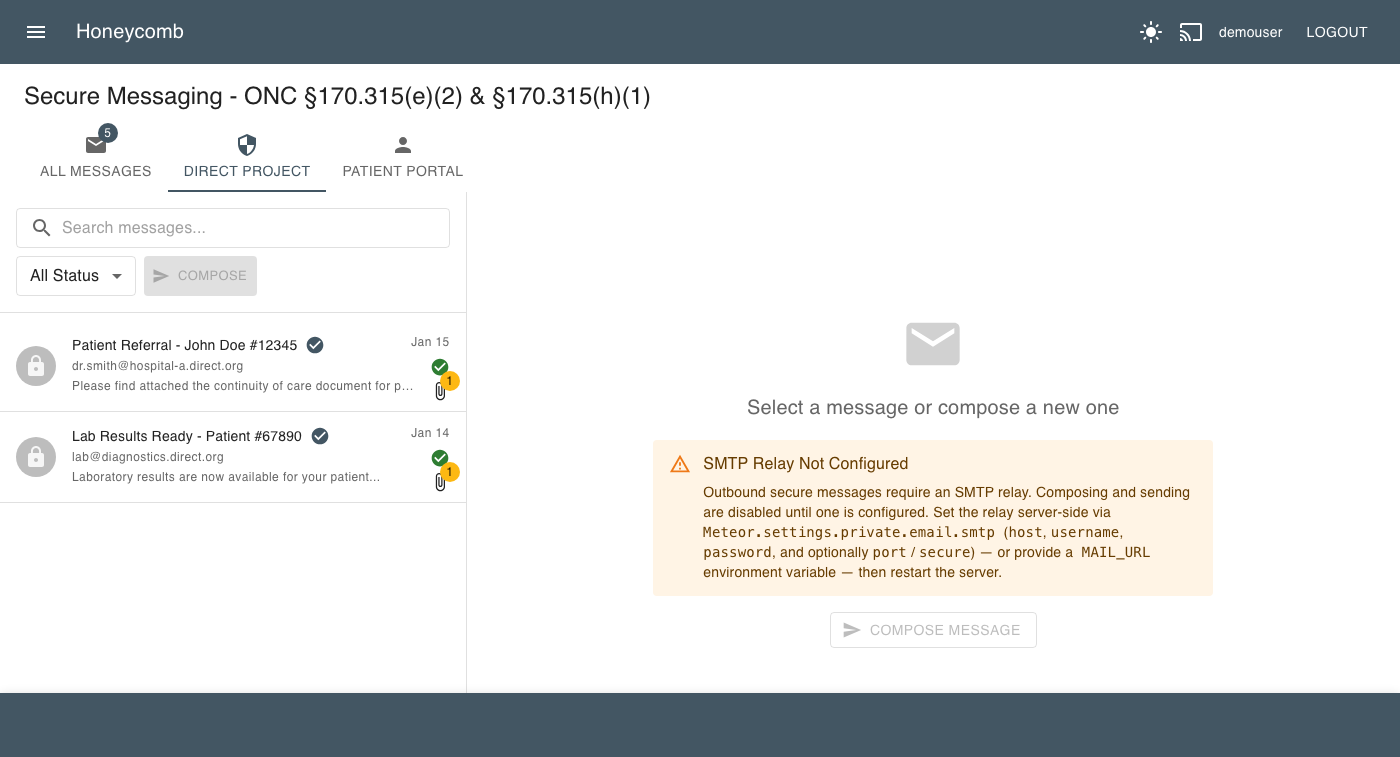
\includegraphics[width=\textwidth]{screenshots/base-ehr_170.315.h.1_direct-project.png}
\caption{Direct Project - Secure Messaging}
\label{fig:h1-screenshot}
\end{figure}

% ============================================================================
\appendix
% ============================================================================

\chapter{Acronyms and Abbreviations}

\begin{description}[style=nextline]
\item[API] Application Programming Interface
\item[BDD] Behavior-Driven Development
\item[C-CDA] Consolidated Clinical Document Architecture
\item[CDS] Clinical Decision Support
\item[CFR] Code of Federal Regulations
\item[CPOE] Computerized Provider Order Entry
\item[DI] Device Identifier
\item[DSI] Decision Support Interventions
\item[EHR] Electronic Health Record
\item[FHIR] Fast Healthcare Interoperability Resources
\item[GMDN] Global Medical Device Nomenclature
\item[GUDID] Global Unique Device Identification Database
\item[HCT/P] Human Cells, Tissues, and Cellular and Tissue-Based Products
\item[HL7] Health Level Seven
\item[MRI] Magnetic Resonance Imaging
\item[OAuth] Open Authorization
\item[ONC] Office of the National Coordinator for Health Information Technology
\item[PI] Production Identifier
\item[SMART] Substitutable Medical Applications, Reusable Technologies
\item[SNOMED CT] Systematized Nomenclature of Medicine - Clinical Terms
\item[SPCU] Sex Parameter for Clinical Use
\item[UDI] Unique Device Identifier
\item[USCDI] United States Core Data for Interoperability
\item[VDT] View, Download, Transmit
\end{description}

\chapter{References}

\begin{enumerate}
\item Office of the National Coordinator for Health Information Technology. \textit{2015 Edition Health IT Certification Criteria, 2015 Edition Base EHR Definition, and ONC Health IT Certification Program Modifications}. 45 CFR Part 170. Federal Register, 2015.

\item Office of the National Coordinator for Health Information Technology. \textit{21st Century Cures Act: Interoperability, Information Blocking, and the ONC Health IT Certification Program}. 45 CFR Part 170. Federal Register, 2020.

\item HL7 International. \textit{FHIR R4 Specification}. http://hl7.org/fhir/R4/

\item HL7 International. \textit{US Core Implementation Guide}. http://hl7.org/fhir/us/core/

\item SMART Health IT. \textit{SMART App Launch Framework}. http://hl7.org/fhir/smart-app-launch/

\item Office of the National Coordinator for Health Information Technology. \textit{United States Core Data for Interoperability (USCDI) Version 5}. 2024.

\item FDA. \textit{Unique Device Identification System (UDI System)}. 21 CFR Part 801.

\item FDA. \textit{Global Unique Device Identification Database (GUDID)}. https://accessgudid.nlm.nih.gov/
\end{enumerate}

\chapter{Certification Testing Notes}

\section{Behavioral Test Suite Status}

Each Base EHR criterion in Part~I has a behavioral Nightwatch test under \texttt{certification/tdd/base\_ehr/} (one file per criterion, \texttt{170.315.<x>.<y>.test.js}). The suite drives real record/change/access behaviors against FHIR resources per the ONC test procedures, not mere page presence, and is run against a live server. As of this revision the outcome is \textbf{11 verified} (green) and \textbf{1 documented gap} (red): (a)(1), (a)(2), (a)(3), (a)(5), (a)(14), (b)(1), (b)(4), (b)(11), (c)(1), (g)(7), and (g)(9) verify; only (h)(1) Direct Project carries a documented gap. Any remaining gaps use explicit \texttt{GAP(170.315.x.y)} annotations that fail deliberately, so the suite functions as a live certification punch-list; the Status column in the Overview and the per-criterion chapters reflect these results. Criterion (g)(10) is covered externally by Inferno (below), not by this suite.

\section{Inferno Testing}

For comprehensive certification testing of the standardized API criterion (g)(10) --- and to authoritatively validate the API surfaces exercised by (g)(7) and (g)(9) --- the official ONC-approved Inferno testing tool must be used. The Inferno (g)(10) suite has been run against this system with passing results; a refreshed run will be executed and formally recorded as part of an ACB submission.

\textbf{Inferno Website:} https://inferno.healthit.gov

Inferno provides authoritative test suites that validate:
\begin{itemize}
\item FHIR R4 conformance
\item US Core Implementation Guide compliance
\item SMART App Launch OAuth 2.0 flows
\item OpenID Connect Core
\item SMART Backend Services (Bulk FHIR)
\item USCDI data completeness
\item Token management and revocation
\item All mandatory and must-support elements
\end{itemize}

The Nightwatch tests in this system provide basic endpoint verification for development and CI/CD purposes. They are \textbf{not} a replacement for Inferno certification testing.

\section{Test Execution}

To run the complete Base EHR test suite:

\begin{Verbatim}[commandchars=\\\{\}]
cd /path/to/core
chmod +x certification/tdd/base_ehr/run-base-ehr-tests.sh
./certification/tdd/base_ehr/run-base-ehr-tests.sh
\end{Verbatim}

Or run a single criterion directly against a running server:

\begin{Verbatim}[commandchars=\\\{\}]
npx nightwatch --config nightwatch.circle.conf.js \\
  certification/tdd/base_ehr/170.315.<x>.<y>.test.js
\end{Verbatim}

The suite covers the twelve in-scope CY2026 Base EHR criteria (one test file each); (g)(10) is intentionally excluded and left to Inferno.

% =====================================================================
% APPENDIX D --- Software Bill of Materials
% =====================================================================
\chapter{Software Bill of Materials (SBOM)}
\label{chap:sbom}

This appendix is the machine-derived Software Bill of Materials for Care
Commons EHR. It is generated from the committed
\texttt{package-lock.json} (\texttt{lockfileVersion~3}) --- the exact
dependency graph resolved for the certification-candidate build --- so it documents the
software as \emph{actually assembled}, not as aspirationally specified. A
complete supply-chain manifest is a deliberate design output: it lets a
reviewer, integrator, or downstream deployer reason about provenance, patch
exposure, and license obligation without treating the system as a black box.

\section{SBOM Metadata}

\begin{center}
\begin{tabular}{@{}ll@{}}
\toprule
\textbf{Field} & \textbf{Value} \\
\midrule
Document format & Dependency manifest (npm \texttt{lockfileVersion 3}) \\
Enumerated on & 2026-07-04 \\
Source of truth & \texttt{package-lock.json} at the certification commit \\
Certification commit & see Reproducibility (\S\ref{sec:reproducibility}) \\
Build runtime (Node) & 22.22.0 (Meteor bundled) \\
Lockfile tooling (npm) & 11.12.1 \\
Framework & Meteor 3.4 \\
Total resolved packages & 4{,}121 \\
Direct dependencies (runtime) & 108 \\
Direct dependencies (dev) & 12 \\
First-party workspace packages & 70 \\
Third-party with SPDX metadata & 4{,}003 \\
Packages without SPDX metadata & 118 \\
\bottomrule
\end{tabular}
\end{center}

\paragraph{Methodology note.} Versions below are reported \emph{exactly as
resolved} in the lockfile. Because Care Commons pins several transitive
dependencies through explicit \texttt{overrides} (for security back-ports)
and runs on the bundled Meteor toolchain, a resolved version may differ from
a package's latest public-registry release. This is expected: the SBOM
records the shipped artifact, which is the artifact put forward for
certification.

\section{Key Components}

The following are the load-bearing third-party components --- the packages a
reviewer most needs to understand. The full transitive set (4{,}121 entries)
lives in \texttt{package-lock.json}; its integrity hash is recorded in the
Reproducibility table (\S\ref{sec:reproducibility}).

\begin{center}
\begin{longtable}{@{}p{0.30\textwidth}p{0.12\textwidth}p{0.34\textwidth}p{0.14\textwidth}@{}}
\toprule
\textbf{Package} & \textbf{Version} & \textbf{Purpose} & \textbf{License} \\
\midrule
\endfirsthead
\toprule
\textbf{Package} & \textbf{Version} & \textbf{Purpose} & \textbf{License} \\
\midrule
\endhead
\bottomrule
\endfoot
\texttt{react} / \texttt{react-dom} & 18.3.1 & UI rendering & MIT \\
\texttt{@mui/material} & 5.18.0 & Component / design system & MIT \\
\texttt{@mui/icons-material} & 5.18.0 & Icon set & MIT \\
\texttt{mongodb} & 6.21.0 & FHIR resource persistence & Apache-2.0 \\
\texttt{express} & 4.22.1 & HTTP / REST routing (FHIR server) & MIT \\
\texttt{@node-oauth/express-oauth-server} & 4.1.5 & OAuth2 authorization server (SMART) & MIT \\
\texttt{jsonwebtoken} & 9.0.3 & JWT signing / verification & MIT \\
\texttt{jose} & 6.2.3 & JWK / JWS / JWE (Backend Services) & MIT \\
\texttt{pkijs} & 3.3.3 & X.509 / PKI (Direct, key material) & BSD-3-Clause \\
\texttt{asn1js} & 3.0.7 & ASN.1 encoding (certificates) & BSD-3-Clause \\
\texttt{dcmjs} & 0.38.3 & DICOM parse / serialize & MIT \\
\texttt{@cornerstonejs/core} & 1.86.1 & Diagnostic image viewing & MIT \\
\texttt{@cornerstonejs/dicom-image-loader} & 1.86.0 & DICOM image loader & MIT \\
\texttt{fqm-execution} & 1.8.5 & FHIR quality-measure engine (c.1) & Apache-2.0 \\
\texttt{xml2js} & 0.6.2 & C-CDA / QRDA XML parse (b.1, c.1) & MIT \\
\texttt{fhirpath} & 4.8.2 & FHIRPath evaluation (search, validation) & Apache-2.0 \\
\texttt{simpl-schema} & 3.4.6 & FHIR resource schema validation & MIT \\
\texttt{lodash} & 4.18.1 & Defensive get/set circuit breaker & MIT \\
\texttt{moment} & 2.30.1 & Date / time handling & MIT \\
\texttt{nightwatch} & 3.14.0 & Behavioral certification E2E tests & MIT \\
\texttt{chromedriver} & 146.0.6 & Headless browser driver (E2E) & Apache-2.0 \\
\texttt{@rspack/core} & 1.7.1 & Workflow-package bundler & MIT \\
\end{longtable}
\end{center}

\section{License Distribution (raw)}

The following is the verbatim SPDX-identifier distribution across all 4{,}003
third-party packages that declare license metadata, as scanned from the
lockfile. It is presented un-normalized for full transparency; the normalized
compliance analysis is in Appendix~\ref{chap:license-compliance}.

\begin{center}
\begin{longtable}{@{}rl@{}}
\toprule
\textbf{Count} & \textbf{SPDX identifier} \\
\midrule
\endfirsthead
\toprule
\textbf{Count} & \textbf{SPDX identifier} \\
\midrule
\endhead
\bottomrule
\endfoot
2919 & MIT \\
283 & Apache-2.0 OR MIT \\
273 & ISC \\
171 & BSD-3-Clause \\
129 & Apache-2.0 \\
70 & UNLICENSED (first-party workspace) \\
40 & 0BSD \\
35 & BSD-2-Clause \\
23 & BlueOak-1.0.0 \\
13 & MPL-2.0 \\
5 & (MIT OR CC0-1.0) \\
5 & (Apache-2.0 OR MIT) \\
4 & Unlicense \\
4 & (MIT AND Zlib) \\
3 & (MIT OR Apache-2.0) \\
3 & (WTFPL OR MIT) \\
2 & SEE LICENSE IN LICENSE.md \\
2 & SEE LICENSE IN LICENSE \\
2 & WTFPL OR ISC \\
2 & (MIT AND BSD-3-Clause) \\
1 & Artistic-2.0 \\
1 & MIT-0 \\
1 & (Unlicense OR Apache-2.0) \\
1 & Python-2.0 \\
1 & CC-BY-4.0 \\
1 & (MIT OR WTFPL) \\
1 & CC0-1.0 \\
1 & (MIT OR GPL-3.0-or-later) \\
1 & LGPL-3.0 \\
1 & (BSD-3-Clause OR GPL-2.0) \\
1 & (BSD-2-Clause OR MIT OR Apache-2.0) \\
1 & WTFPL \\
\end{longtable}
\end{center}

% =====================================================================
% APPENDIX E --- License Compliance Report
% =====================================================================
\chapter{License Compliance Report}
\label{chap:license-compliance}

This appendix normalizes the raw distribution in Appendix~\ref{chap:sbom}
into license \emph{families}, states the obligation each family imposes, and
records how those obligations interact with Care Commons EHR's own
distribution license. The headline finding: the dependency tree is overwhelmingly
permissive (roughly 96\% MIT / ISC / BSD / Apache / public-domain-equivalent),
carries no imported strong-copyleft (GPL/AGPL) obligation, and every
copyleft component present is either file-level (MPL-2.0) or weak
(LGPL-3.0) and used in a compatible way.

\section{The Application's Own License}

The Care Commons EHR application code is licensed \textbf{AGPL-3.0} (see
\texttt{LICENSE.md}). This is an intentional network-copyleft posture: an
operator running a modified Care Commons EHR as a network service must offer
that modified source to its users. AGPL-3.0 is the \emph{outbound} license of
the first-party application; it is not imposed by any dependency. The workflow
packages under \texttt{npmPackages/} are individually MIT (or Apache-2.0 for
the core subset); private packages under \texttt{extensions/} are
\texttt{UNLICENSED} and are not distributed with the open-source release.

\section{License Families and Obligations}

\begin{center}
\begin{longtable}{@{}p{0.30\textwidth}rp{0.34\textwidth}c@{}}
\toprule
\textbf{Family} & \textbf{Count} & \textbf{Obligation} & \textbf{Compat.} \\
\midrule
\endfirsthead
\toprule
\textbf{Family} & \textbf{Count} & \textbf{Obligation} & \textbf{Compat.} \\
\midrule
\endhead
\bottomrule
\endfoot
MIT / ISC / 0BSD / BSD-2 / BSD-3 / BlueOak & 3462 & Preserve copyright + license text (attribution) & \checkmark \\
Apache-2.0 (incl.\ Apache/MIT dual) & 420 & Preserve NOTICE; explicit patent grant & \checkmark \\
Public-domain-equivalent (Unlicense, CC0, MIT-0) & 12 & None & \checkmark \\
Other permissive dual/combos (Zlib, WTFPL, Python-2.0, \ldots) & 16 & Attribution where applicable & \checkmark \\
MPL-2.0 & 14 & File-level source disclosure for \emph{modified} MPL files only & \checkmark \\
LGPL-3.0 & 1 & Allow relinking; provide LGPL source (dynamic use) & \checkmark \\
Dual-with-GPL (resolve to permissive side) & 2 & Elect the non-GPL option (MIT / BSD) & \checkmark \\
CC-BY-4.0 & 1 & Attribution (asset / data, not code) & \checkmark \\
Artistic-2.0 & 2 & Attribution; state changes & \checkmark \\
Custom (``SEE LICENSE IN\ldots'') & 5 & Manual review of bundled LICENSE file & review \\
UNLICENSED (first-party workspace) & 70 & N/A --- own code (AGPL / MIT / private) & --- \\
No SPDX metadata & 118 & Mostly \texttt{@types} stubs + first-party; reviewed & low \\
\bottomrule
\end{longtable}
\end{center}

\section{Attribution and Notice Obligations}

\begin{itemize}
\item \textbf{Permissive attribution (MIT/BSD/ISC).} The largest obligation
  by count is simple attribution: the copyright notice and license text of
  each package must travel with any redistribution. These are preserved in
  each package's own \texttt{LICENSE} file within \texttt{node\_modules} and
  are reproduced in binary/desktop distributions.
\item \textbf{Apache-2.0 NOTICE.} Apache-2.0 packages that ship a
  \texttt{NOTICE} file require that file to be preserved and passed through;
  Apache-2.0 also grants an explicit patent license, which is favorable for a
  regulated deployment.
\item \textbf{MPL-2.0 (file-level copyleft).} MPL is per-file: only if a
  specific MPL-licensed \emph{source file} is modified must that file's source
  be offered. Care Commons consumes these packages unmodified, so the only
  obligation is to preserve their license headers. MPL-2.0 \S3.3 is explicitly
  compatible with (A)GPL distribution.
\item \textbf{LGPL-3.0 (weak copyleft).} The single LGPL component is used as
  a dynamically-resolved library, satisfying the relinking allowance; its
  source is available upstream.
\item \textbf{Dual-licensed with a GPL option.} Two packages offer a choice
  that includes a GPL variant; Care Commons elects the permissive alternative
  (MIT / BSD-3-Clause), so no GPL obligation attaches.
\end{itemize}

\section{Source Availability}

Because the application is AGPL-3.0, corresponding source for the first-party
code is made available with every network deployment. Third-party source is
obtainable from each package's public repository (recorded in
\texttt{package-lock.json} \texttt{resolved} URLs); nothing in the tree is a
proprietary binary blob requiring a separate source-offer letter.

\section{Findings}

\begin{enumerate}
\item \textbf{No imported strong copyleft.} There is no GPL-2.0-only or
  GPL-3.0-only or AGPL \emph{dependency} in the tree. The only AGPL in the
  system is Care Commons EHR's own outbound license.
\item \textbf{No external UNLICENSED risk.} All 70 \texttt{UNLICENSED}
  entries are first-party workspace packages (verified: every one resolves
  to \texttt{npmPackages/}, \texttt{extensions/}, or \texttt{core/} via a
  workspace symlink). None is an unlicensed third-party import.
\item \textbf{Copyleft is bounded.} The 14 MPL-2.0 and 1 LGPL-3.0 components
  impose only file-level / relinking obligations, all satisfied by unmodified
  dynamic use.
\item \textbf{Flagged for periodic manual review.} 5 ``SEE LICENSE'' custom
  declarations and 118 metadata-absent packages (predominantly
  \texttt{@types} stubs, which are non-executable) should be re-examined on
  each major dependency bump. None is currently believed to impose a
  restrictive obligation.
\end{enumerate}

\section{Open-Source Provenance}

Beyond ``which licenses,'' the more useful transparency question is
\emph{why each major component exists}. The table below turns the dependency
list into an architectural map, so a reviewer can see the system as an
intentional assembly of well-understood parts.

\begin{center}
\begin{longtable}{@{}p{0.36\textwidth}p{0.58\textwidth}@{}}
\toprule
\textbf{Component} & \textbf{Reason it is in the system} \\
\midrule
\endfirsthead
\toprule
\textbf{Component} & \textbf{Reason it is in the system} \\
\midrule
\endhead
\bottomrule
\endfoot
Meteor 3.4 (runtime) & Full-stack framework: DDP transport, reactive data, build toolchain \\
React + React-DOM & Client UI rendering \\
Material-UI (MUI) & Component library and light/dark design system \\
MongoDB driver & Document persistence for FHIR resources \\
Express & HTTP surface for the FHIR REST API \\
@node-oauth/express-oauth-server & OAuth2 authorization server for SMART App Launch \\
jsonwebtoken + jose & JWT / JWK handling for SMART and Backend Services \\
pkijs + asn1js & X.509 / certificate handling for the Direct transport and key material \\
dcmjs & DICOM parsing and serialization \\
Cornerstone3D & Diagnostic image viewing \\
fqm-execution & FHIR Clinical Quality Measure calculation (\S170.315(c)(1)) \\
xml2js & C-CDA and QRDA XML parsing (\S170.315(b)(1), (c)(1)) \\
fhirpath & FHIRPath evaluation for search and validation \\
simpl-schema & FHIR resource schema validation \\
Nightwatch & Behavioral compliance (E2E) testing \\
Inferno (external) & ONC-approved standardized-API conformance testing (\S170.315(g)(10)) \\
\end{longtable}
\end{center}

\section{Reproducible Build}

So that another engineer can recreate the exact tree audited above, the
canonical build coordinates are recorded once in the Reproducibility table
(\S\ref{sec:reproducibility}) and summarized here: Git commit SHA,
\texttt{package-lock.json} SHA-256 integrity hash, Node 22.22.0, npm 11.12.1,
Meteor 3.4, MongoDB 7.0.16 (dev) / 6.0 (CI), on macOS / Linux. Restoring that
lockfile with \texttt{npm ci} yields a byte-identical dependency graph, and
therefore an SBOM identical to this one.
